 % !TEX root = Stanfill_CoDA.tex
\appendix

\section{Sampling Process}
\label{sec:appendix1}
\subsection{Circular-von Mises-based distribution}

To simulate a set of random rotations from the circular-von Mises-based distribution we follow the  algorithm proposed by \citet{best79}.  The algorithm is available in the IMSL Library (1991) and is implemented as follows.  Let $\mu=0$ denote the mean of the target angular distribution and $\kappa$ its concentration parameter.  We define constants $a, b$ and $d$ as
$a\equiv 1+\sqrt{1+4\kappa^2},\quad b\equiv(a-\sqrt{2a}),\quad d\equiv(1+b^2)/2b.$
In steps one, two and four we generate three new observations $u_1$, $u_2$ and $u_3$,  each from a uniform distribution defined over the interval $(0,1)$. 
\begin{enumerate}
\item Set $z=\cos(\pi u_1)$, $f=(1+dz)/(z+d)$ and $c=\kappa(d-f)$.
\item If $c(2-c)-u_2>0$ go to step 4.
\item If $\log(c/u_2)+1-c<0$ return to step 1.
\item Set $r=\text{sign}(u_3-0.5)\cos^{-1}(f)$
\item Then $r$ follows a von Mises $(\kappa)$ distribution.
\end{enumerate}

\subsection{Cayley distribution}\hfill

To simulate rotation matrices from a Cayley distribution we make use of a result given in \citet{leon06}. If the angle $r$ follows a Cayley distribution it holds that $\frac{1+\cos r}{2} \sim \text{Beta}(\kappa+1/2, 3/2)$.  Hence, angles according to a Cayley distribution can be simulated through composition: we simulate a Bernoulli trial $Y$ with outcomes -1 and 1 having probability 0.5 and an observation $X$ from a Beta$(\kappa+1/2, 3/2)$ distribution and then set $r= \frac{Y}{2}\cos^{-1}(2X-1)$. 

\subsection{matrix Fisher distribution}\hfill

Simulation from the matrix Fisher distribution is achieved through a rejection algorithm.  Let  $\mathrm{C_F}(r|\kappa)$ denote the matrix von Mises-Fisher density as given in Table~\ref{tab:ang.dens} and $Y\sim$ Uniform$(-\pi,\pi]$.

\begin{enumerate}
\item Define $M=\frac{1}{2\kappa}e^{2\kappa - 1}\frac{1}{\mathbf{I}_0(2\kappa)-\mathbf{I}_1(2\kappa)}$
\item Generate $U\sim$ Uniform$(0,1)$ and $Y\sim$ Uniform$(-\pi,\pi]$, where $U$ and $Y$ are independent.
\item If $U<\frac{1}{M}\mathrm{C_F}(Y|\kappa)$, accept $Y$; otherwise return to step (2)
\end{enumerate}

Given a set of randomly generated angles $r_1,\ldots, r_n$ we can now generate the corresponding set of rotation matrices as follows:
\begin{enumerate}
\item Generate a point uniformly on the unit sphere
$$\bm{U}=(u_1,u_2,u_3)^\top=(\sin\theta\cos\phi,\sin\theta\sin\phi,\cos\theta)^\top$$
where  $0\leq \theta\leq \pi$ and $0\leq \phi\leq 2\pi$.
\item Given an angle of rotation, $r_i$, generated as described above from an angular distribution symmetric about 0 and with concentration $\kappa$ rotate $\bm{I}$ about $\bm{U}$ by $r_i$ radians.
\end{enumerate}

\subsection{Comparison of Euclidean and Riemannian Metrics When Measuring Distance to the Central Direction}\hfill\\

The results section of this paper only compared the distances of each estimator from the central direction in terms of Riemannian distance.  This section is intended to show that a comparison based on the Euclidean distance will not lead to different results.  Recall that the Riemannian distance between two rotations is the shortest geodesic curve that connects those two rotations and the Euclidean distance is the shortest cord that connects those two rotations.  Refer to the picture below for a two-dimensional simplification of the idea.

%\begin{center}
%\begin{tikzpicture}
%\draw (0,0) circle (4cm);
%\draw (0,0)--(4,0) node[anchor =  west]{$\bm R_1$};
%\draw (0,0)--(-2,3.46) node[anchor = south east]{$\bm R_2$};
%\draw[line width=.75mm] (4,0) arc (0:120:4cm);
%\draw[line width=.75mm, color=gray] (-2,3.46)--(4,0);
%\draw (0,0)--(2,3.46) node[anchor= south west]{$\alpha$};
%\draw (3/8,.7)[->] arc (60:120:.75cm);
%\draw (0,1.2) node {$\frac{\alpha}{2}$};
%\draw (0,2.8) node {$\frac{\beta}{2}$};
%\draw (2,0) node[anchor=north]{1};
%\end{tikzpicture}
%\end{center}

%\begin{figure}[h!]
\begin{center}
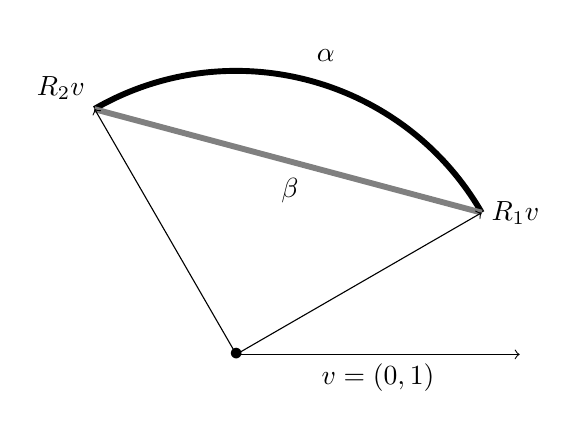
\begin{tikzpicture}[scale=.9]
%\draw (0,0) circle (4cm);
\draw (0,0) node {$\bullet$};
\draw (3.464102,2) node[anchor =  west]{$\bm R_1\bm v$};
\draw [->] (0,0)--(4,0);
%\draw [->] (4,0) arc (0:30:4cm);
\draw (2,0) node[anchor = north]{$\bm v=(0,1)$};
\draw (-2,3.46) node[anchor = south east]{$\bm R_2\bm v$};
\draw [line width=.75mm] (3.464102,2) arc (30:120:4cm);
\draw[line width=.75mm, color=gray] (-2,3.46)--(3.464102,2);
\draw [->](0,0) -- (-2,3.464102);
\draw [->](0,0)--(3.464102,2);
\draw (1,4) node[anchor= south west]{$\alpha$};
\draw (.5,2) node[anchor= south west]{$\beta$};
%\draw (0,0) circle (4cm);
%\draw (0,0) node {$\bullet$};
%\draw (0,0)--(4,0) node[anchor =  west]{$o_1$};
%\draw (4,0) node[anchor =  west]{$\bm R_1$};
%\draw (0,0)--(-2,3.46) node[anchor = south east]{$o_2$};
%\draw (-2,3.46) node[anchor = south east]{$\bm R_2$};
%\draw[line width=.75mm] (4,0) arc (0:120:4cm);
%\draw[line width=.75mm, color=gray] (-2,3.46)--(4,0);
%\draw (0,0)--(2,3.46) node[anchor= south west]{$\alpha$};
%\draw (2,3.46) node[anchor= south west]{$\Rdist (\bm R_1,\bm R_2)$};
%\draw (-1.25,0.73) node[anchor= south west]{$\Edist (\bm R_1,\bm R_2)$};
%\draw (3/8,.7)[->] arc (60:120:.75cm);
%\draw (0,1.2) node {$\frac{\alpha}{2}$};
%\draw (0,2.8) node {$\frac{\beta}{2}$};
%\draw (2,0) node[anchor=north]{1};
\end{tikzpicture}
\end{center}
%\caption{An illustration of the difference between the Euclidean and Riemannian distance metrics on $SO(2)$.}
%\label{fig:dEvsdG} 
%\end{figure}
\section{No Name yet}
\label{sec:appendix2}
Let $\bm R_1\bm v$ and $\bm R_2\bm v$ be two observations in $SO(2)$.  The Riemannian distance between these two observations is given by $\alpha$ and is indicated with the thick black arc.  The Euclidean distance is given by $\beta$ and is indicated by the gray line running through the circle.  Because this is the unit circle, the Riemannian distance is also the angle in the center of the circle thus, using basic geometry its clear that half of the Euclidean distance is the sine of half of the Riemannian distance, i.e.
\[
\beta=2\sin\left(\frac{\alpha}{2}\right).
\]

Extending this to $SO(3)$ gives the following proposition: for all $\bm{R}_1$ and $\bm{R}_2$ in $SO(3)$
\begin{equation}\label{EvR}
\Edist (\bm{R}_1,\bm{R}_2)=2^{3/2}\sin\left(\frac{\Rdist(\bm{R}_1,\bm{R}_2)}{2}\right).
\end{equation}
\emph{Proof:}\\
Let $\bm{o}_1,\bm{R}_2\in SO(3)$ be given and define $\tr(\bm R_1^\top\bm R_2)=1+2\cos(\theta)$ then $|\theta|=\Rdist(\bm R_1,\bm R_2)$.  Notice that \eqref{EvR} holds trivially for $\Edist (\bm R_1,\bm R_2)=\Rdist(\bm R_1,\bm R_2)=0$ so consider the case $|\theta|>0$.  By definition of $\Edist (\bm R_1,\bm R_2)$ we have the following:
\begin{align*}
\Edist (\bm R_1,\bm R_2)^2
&=||\bm R_1-\bm R_2||_F^2\\
&=\tr\left[(\bm R_1-\bm R_2)^\top(\bm R_1-\bm R_2)\right]=\tr\left[(\bm R_1^\top-\bm R_2^\top)(\bm R_1-\bm R_2)\right]\\
&=\tr\left[\bm R_1^\top\bm R_1+\bm R_2^\top\bm R_2-\bm R_2^\top\bm R_1-\bm R_1^\top\bm R_2\right]\\
&=\tr\left[2\bm{I}-\bm R_2^\top\bm R_1-\bm R_1^\top\bm R_2\right]\\
&=2\tr(\bm{I})-\tr(\bm R_2^\top\bm R_1)-\tr(\bm R_1^\top\bm R_2)\\
&=6-2\tr(\bm R_1^\top\bm R_2)=6-2(1+2\cos(\theta))\\
&=6-2-4\cos(\theta)=8\left(\frac{1-\cos(\theta)}{2}\right)\\
&=8\sin^2\left(\frac{\theta}{2}\right)\\
&=\left[2^{3/2}\sin\left(\frac{|\theta|}{2}\right)\right]^2\\
&=\left[2^{3/2}\sin\left(\frac{\Rdist(\bm R_1,\bm R_2)}{2}\right)\right]^2
\end{align*}
Taking square roots on both sides and noticing that $\Edist (\bm R_1,\bm R_2)\geq0$ and $\Rdist (\bm R_1,\bm R_2)\geq0$ gives \eqref{EvR}.\\
$\Box$
